%!TEX root = ../template.tex
%%%%%%%%%%%%%%%%%%%%%%%%%%%%%%%%%%%%%%%%%%%%%%%%%%%%%%%%%%%%%%%%%%%%
%% chapter4.tex
%% NOVA thesis document file
%%
%% Chapter with lots of dummy text
%%%%%%%%%%%%%%%%%%%%%%%%%%%%%%%%%%%%%%%%%%%%%%%%%%%%%%%%%%%%%%%%%%%%

\typeout{NT FILE chapter4.tex}%

\chapter{Background}
\label{cha:background}

In this section, the technology behind the development and deployment of a microservices-based
application system will be described using the underlying design principles.

\section{Microservices} % (fold)
\label{sec:microservices}

[Hassan et al. 2017]
[Aderaldo et al. 2017]
https://martinfowler.com/articles/microservices.html

Microservices are an architectural style in which software is developed using self-contained components that
communicate with one another via standardized interfaces and lightweight mechanisms.
These services segregate fine-grained business functionalities and can be independently deployed, scaled, and tested by fully automated machinery.
There is a bare minimum of centralized management, and each service may be written in a different programming language and use different data storage technologies.

\paragraph{}

To understand the microservice style it's useful to compare it to the monolithic style:
A monolithic application is built often using the Model-View-Controller (MVC) pattern, which is divided in three main parts:
The view, a client-side user interface, consisting of HTML pages and javascript running in a browser on the user's machine.
The model, a relational database management system,
The controller, a server-side application that handles requests, execute domain logic, retrieve and update data from the database, and selects and populates the views to be sent to the browser.

\paragraph{}

This server-side application is a monolith a single logical executable, in which all logic for handling requests runs as a single process,
different domains of the application are divided into classes, functions, and namespaces by utilizing the basic features of a programming language.

When monolithic applications need to scale and maintain a high level of availability, they become a source of frustration.
Any small change made to the server-side application, involves building and re-deploying the entire monolith.
Scaling the server-side application involves scaling all the application functionalities, rather than the functionalities that require greater resources.

\begin{figure}[htbp]
    \centering
    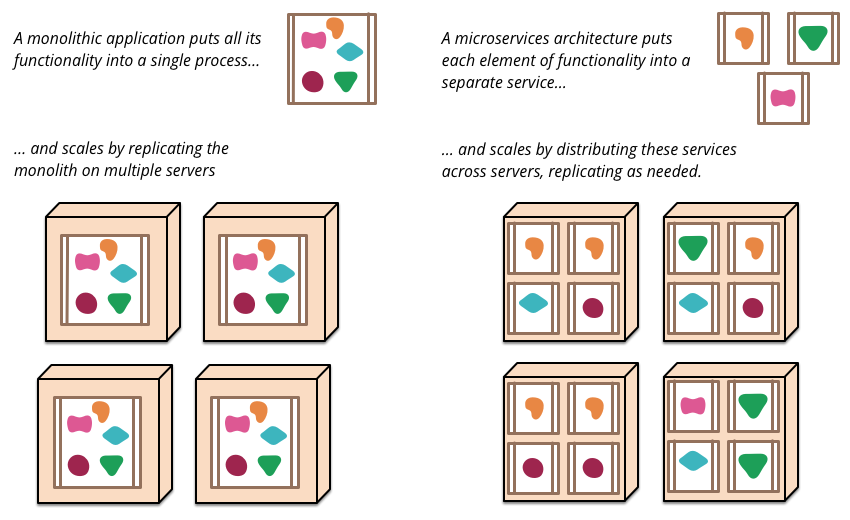
\includegraphics[height=3in]{microVSmono}
    \caption{Monoliths and Microservices}
    \label{fig:monoliths and microservices}
\end{figure}

The requirements of system scalability, high availability, and continuous delivery are addressed in different microservice architectural characteristics.

\paragraph{Componentization}

In contrast to monoliths, which achieve componentization solely via the use of libraries and programming language capabilities,
microservices achieve componentization primarily through the division of different business domains and functionalities into distinct executables
that are exposed as services.

While this componentization approach helps to enforce component's encapsulation via more explicit component interfaces,
its primary benefit is that services become independently deployable.
This feature helps to fulfill the requirements of system scalability and high availability by
making different components scalable across multiple nodes and limiting cascading errors via the replication and isolation of components.

\paragraph{Decentralized Data Management}

While monolithic applications typically use a single logical database for persistent data,
microservices offer higher flexibility, fault-tolerance and scalability by letting each service manage its own database, either different instances of the same database technology,
or entirely different database systems.
Decentralizing the responsibility for data across different services has implications in the implementation of cross-domain operations that affect multiple resources.
The common approach for dealing with this problem in database systems is to use transactions to guarantee consistency when updating multiple resources.
Building and maintaining applications that use transactions in a distributed setting is notoriously difficult,
as a result, microservice architectures emphasize transaction-less coordination between services,
with explicit recognition that consistency may only be eventual consistency and problems are dealt with by compensating operations.


\paragraph{Inter-process Communication Strategies}

Martin Fowler, a well-known author in the context of microservices, advocates what he calls "smart endpoints and dumb pipes" for microservices communication.
Enterprise Service Buses (ESB) were previously frequently used in service-oriented architecture (SOA) systems,
and it was common to incorporate orchestration and transformation logic into the communication infrastructure,
making the pipe "smart." There were multiple problems with this approach:
the tooling was complex and expensive, and it was difficult to troubleshoot when problems occurred in production environments.

The reverse approach has been adopted with microservices,
where services own their domain-centric logic "smart endpoints" and use "dumb pipes" as a transport method.
The majority of communication between microservices is done via request/response-based communication or event-driven messaging.
Because these two methods have such dissimilar properties, it's important to weigh their strengths, and the scenarios that call for each.

Request/response-based communication protocols are typically suited for synchronous settings,
where the client contacts one receiver at time and needs the response before it can continue.
In this approach there is a clear control of the flow,
there is a service that plays the role of orchestrator and determines the sequence of operations to be performed in other services.
The HTTP and RPC protocols are the most widely adopted protocols that follow this approach.

Event-driven messaging communication protocols are suited for asynchronous settings,
where the client publishes a message to multiple receivers and can process the responses at a later time.
In this approach there is no orchestrator, each service knows their role and what to do based on events that occurred.
The main disadvantage of this strategy is that consistency is not guaranteed when multiple services consume events and one of them fails.

\paragraph{Evolutionary Design}
When decomposing a software system into components, we must decide how to divide the pieces.
The concept of independent replacement and upgrade-ability are critical properties when designing component.
The disadvantage of incorporating components into services is that we must be concerned about changes to one service breaking its consumers.
The traditional integration approach is to attempt to resolve this issue through the use of versioning.
In the context of microservices, versioning entails the maintenance of multiple deployments of the same service in distinct versions.
We can minimize the use of versioning by designing services in such a way that they are as tolerant as possible to supplier changes,
utilizing techniques such as Domain-Driven Design (DDD).
DDD is a software design approach that decomposes a complex system into multiple autonomous bounded contexts,
where all the structure and language of software (class names, class methods, class variables) match the business domain.

\section{Microservice Lifecycle Management} % (fold)
\label{sec:microservice_lifecycle_management}

To run microservices in the cloud, we need two essential ingredients a method for packaging and isolating services,
and a management system capable of provisioning physical hardware to support them.

\paragraph{}

The isolation of services is accomplished through resource virtualization in one of two ways: containers or virtual machines (VM).

Containers provide the most efficient approach because unlike VMs, containers share the host system’s kernel with other containers.
VMs virtualize an entire machine down to the hardware layers, while containers only virtualize software layers above the operating system level.

Docker is the most popular container technology. It is built on top of the following technologies: Kernel namespaces, Cgroups, Copy-on-write File system.
\begin{itemize}
    \item Namespaces: Isolate the kernel resources (processes, filesystem, users, network stacks, \ldots) used by each container.
    \item Cgroups: Isolate the hardware resources used by each container.
    \item Copy-On-Write File system: Allows several containers to share common data.
\end{itemize}

Additionally, Docker provides a mechanism for packaging code and its dependencies, referred to as container images.
A container image is a lightweight, standalone executable package of software that contains all the components necessary to run an application: code, libraries, runtime and settings.

\paragraph{}

The management of services can be accomplished with the use container orchestration technologies.
Container orchestration eliminates many of the manual processes involved in the management of distributed systems.
Some popular options used for the lifecycle management of services are Docker Swarm and Kubernetes.

Kubernetes is an open-source container orchestration system that evolved from Google's Borg and Omega projects.
Kubernetes is an ambitious platform. It manages the deployment, management, scaling, and networking of containers of distributed systems across a wide range of environments
and cloud providers.

This means ensuring that all containers used to execute various workloads are scheduled to run on physical or virtual machines,
while adhering to the deployment environment's and cluster configuration's constraints.
Any containers that are dead, unresponsive, or otherwise unhealthy are automatically replaced.
Additionally, Kubernetes also provides a control plane to monitor all running containers.

Kubernetes accomplishes this through a well-defined, high-level architecture that encourages extensibility:

\begin{itemize}
    \item Pod: Encapsulates an application's container (or multiple containers),
    storage resources, haves a unique network IP address, and provides configuration options for the container(s).
    \item Service: Is an abstraction which defines a logical set
    of Pods and a policy by which to access them.
    \item Volume: Is a directory which is accessible to the
    Containers in a Pod.
    \item Namespace: Provide a scope for names. Names
    of resources need to be unique within a namespace, but not
    across namespaces.
    \item Deployment: Describes the desired state of the system. The
    Deployment Controller changes the actual state to the desired
    state at a controlled rate.
    \item ReplicaSet: Ensures that a specified number of pod replicas
    are running at any given time.
    \item DaemonSet: ensures that all (or some) Nodes run a copy of
    a Pod.
    \item StatefulSet: Is used to manage stateful applications.
\end{itemize}

Kubernetes is a more sophisticated container management system than Docker Swarm.
Docker Swarm is only compatible with Docker, whereas Kubernetes is compatible with other container services.
In comparison to Swarm, Kubernetes is more difficult to deploy and manage, however is said to be more scalable.

\section{TypeSafe Contract Evolution in MicroService Architectures} % (fold)
\label{sec:typesafe_contract_evolution_in_microservice_architectures}


Our framework is inspired by the programming model of the OutSystems Platform,
a low-code platform based on visual languages, for the development of enterprise-
grade mobile and web applications that abstracts and manages most of the technical
details of deploying and maintaining cloud-based data-centric applications. The results
of this paper lay the ground for future versions of the platform that automatically
and seamlessly will distribute programming modules using microservices instead of
heavyweight web containers.
In summary, the contributions of this paper are the following:
A model for an integrated lifecycle management system targeting a microservices
infrastructure;
A compatibility relation on service contracts, based on real traces of evolution, that
ensures that it is always possible to generate adapter code for values of compatible
types;
An adaptation protocol flexible enough to transfer data between different (but
compatible) versions of services without losing data (lemma 6);
A semantics for a microservice management system whose operations include
remote calls between services, deployment and undeployment of services;
A type based structuring discipline for microservices, and a corresponding lightweight
preflight check procedure for deployment operations. The type soundness result
(theorem 1) certifies the safety of the deployment operations.


We present a microservice management system that statically verifies service interface signatures against
their references and supports the seamless evolution of compatible interfaces.

We define a compatibility relation on types that captures real evolution patterns and embodies known good practices on the evolution of
interfaces.

Namely, we allow for addition, removal, and renaming of data fields of a producer module without
breaking or needing to upgrade consumer services.

The evolution of interfaces is supported by runtime generated proxy components that dynamically adapt data exchanged between services to match with the statically
checked service code.

The model proposed in this paper is instantiated in a core programming language whose semantics is
defined by a labelled transition system and a type system that prevents breaking changes from being deployed.

Standard soundness results for the core language entail the existence of adapters, and hence ensure the
absence of adaptation errors and the correctness of the management model.

This adaptive approach allows for gradual deployment of modules, without halting the whole system and avoiding losing or misinterpreting
data exchanged between system nodes.

Experimental data shows that an average of 57\% of deployments that would require adaptation and recompilation are safe under our approach.


Our research is motivated by data from real, large-scale, applications created with
the OutSystems platform. The evaluation of our model presented in this section is
twofold. In a first assessment, we gather data from real applications and analyse the
traces of past deployments (5 years) under our evolution model to measure its impact.
In a second phase, we compare the actual evolution of an OutSystems application
before and after the adoption of our compatibility model between module references.

We have defined a principled evolution mechanism that accounts for deployments
that correspond to what should be compatible interface evolutions and nevertheless
usually force the redeploy (and corresponding downtime) of consumer modules.
We address the problem of service interface evolution in a loosely-coupled setting,
targeting increased deployment flexibility. We present a language-based lifecycle
management model for microservice-based systems that statically checks new service
versions, preventing breaking deployments, and certifying the capability of the system
to adapt to compatible changes. Also, the system’s compatibility algorithm supports
several common changes as compatible: adding, reordering and renaming fields.
These compatibility scenarios are supported by a runtime adaptation protocol that
generates specialised proxies for each producer, ensuring that no communication
errors or data loss ever occurs. The flexibility introduced by the referred compatibility
relation is framed by the automatic proxy generation. We guaranty that adaptation
code is always defined for all pairs of compatible types. The soundness of the type
system implies that well defined deployments don’t break the system (theorem 1). Our
experimental evaluation (section 9) shows significant improvements on the number
of independent deployments in real applications that do not require intervention in
consumer modules, corresponding to at least 57 % of all deployments with interface
changes.